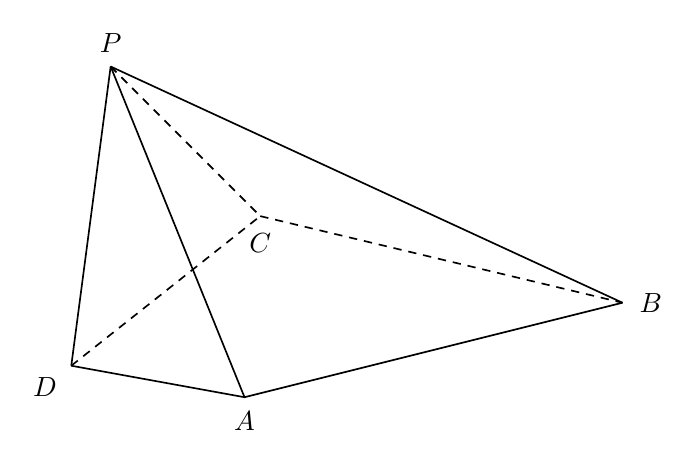
\begin{tikzpicture}[x=1cm,y=1cm,font=\normalsize]
\tikzset{se/.style={solid,line width=.6pt},he/.style={dashed,line width=.6pt,dash pattern=on 3pt off 2.5pt}}
\coordinate (P) at (0.5,4.2);
\coordinate (D) at (0,0.4);
\coordinate (A) at (2.2,0);
\coordinate (B) at (7.0,1.2);
\coordinate (C) at (2.4,2.3);
% hidden edges
\draw[he] (P) -- (C);
\draw[he] (D) -- (C);
\draw[he] (C) -- (B);
% visible edges
\draw[se] (P) -- (D);
\draw[se] (P) -- (A);
\draw[se] (P) -- (B);
\draw[se] (D) -- (A) -- (B);
\node[inner sep=2pt,font=\normalsize,above,yshift=3pt] at (P) {$P$};
\node[inner sep=2pt,font=\normalsize,below left,xshift=-3pt,yshift=-2pt] at (D) {$D$};
\node[inner sep=2pt,font=\normalsize,below,yshift=-3pt] at (A) {$A$};
\node[inner sep=2pt,font=\normalsize,right,xshift=4pt] at (B) {$B$};
\node[inner sep=2pt,font=\normalsize,below,yshift=-4pt] at (C) {$C$};
\end{tikzpicture}
